% This is the University of Chicago Graham School Master of Science in Analytics
% template. Much of it is based on the Reed College LaTeX thesis template.
% Most of the work for the Reec College template was done by Sam Noble (SN),
% Later comments etc. by Ben Salzberg (BTS).
% Additional restructuring and APA support by Jess Youngberg (JY).
% Justin M. Shea (JMS) built on their good open source work.
% Your comments and suggestions are more than welcome:
% please email, them to justinshea@uchicago.edu.
%
% Any line that starts with a percent symbol is a comment.
% They won't show up in the document, and are useful for notes
% to yourself and explaining commands.
% Commenting also removes a line from the document;
% very handy for troubleshooting problems. -BTS
%%
%% Preamble
%%
% \documentclass{<something>} must begin each LaTeX document
% Added by JMS
\documentclass[12pt,oneside]{chicagocapstone}
% END of JMS add
% Packages are extensions to the basic LaTeX functions. Whatever you
% want to typeset, there is probably a package out there for it.
% Check out CTAN to see: http://www.ctan.org/
%%
\usepackage{graphicx,latexsym}
\usepackage{amsmath}
\usepackage{amssymb,amsthm}
\usepackage{longtable,booktabs,setspace}
\usepackage[hyphens]{url}
% Added by CII
\usepackage{hyperref}
\usepackage{lmodern}
\usepackage{float}
\floatplacement{figure}{H}
% End of CII addition
\usepackage{rotating}


% Added by CII (Thanks, Hadley!)
% Use ref for internal links
\renewcommand{\hyperref}[2][???]{\autoref{#1}}
\def\chapterautorefname{Chapter}
\def\sectionautorefname{Section}
\def\subsectionautorefname{Subsection}
% End of CII addition

% Added by CII
\usepackage{caption}
\captionsetup{width=5in}
% End of CII addition

% Added by JMS
\usepackage{mathptmx} % Times New Roman fonts
% End of add by JMS

% Syntax highlighting #22

% To pass between YAML and LaTeX the dollar signs are added by CII
\title{Music Generator}
\author{Terry Wang, Rima Mittal, Joshua Goldberg}
\date{March, 2020} % The month and year that you submit your FINAL draft)
\division{Graham School}
\advisor{Yuri Balasanov}
\institution{University of Chicago}
\degree{Master of Science in Analytics}
% End of CII addition

\department{Continuing Liberal and Professional Studies}

% Added by CII
%%% Copied from knitr
%% maxwidth is the original width if it's less than linewidth
%% otherwise use linewidth (to make sure the graphics do not exceed the margin)
\makeatletter
\def\maxwidth{ %
  \ifdim\Gin@nat@width>\linewidth
    \linewidth
  \else
    \Gin@nat@width
  \fi
}
\makeatother

\renewcommand{\contentsname}{Table of Contents}
% End of CII addition

\setlength{\parskip}{0pt}

% Added by CII
  %\setlength{\parskip}{\baselineskip}
  \usepackage[parfill]{parskip}

\providecommand{\tightlist}{%
  \setlength{\itemsep}{0pt}\setlength{\parskip}{0pt}}


\Abstract{
We propose the application of Deep Learning models to help individuals generate interesting music ideas. The platform has a GAN-based generator. The data used to train the generator are 130,000 midi files across many different genres of music. The algorithmic process is expected to be able to explore more music combinations than any individual, and thus provide a more holistic and creative approach to music creation.

Our work includes a modified version of the python package pretty\_midi, which serves as a midi pre-processing starter package for Deep Learning. Using Generative Adversarial models, we provide insights on predicting pitches and duration to ultimately generate music notes.

\bigskip 
\bigskip
\bigskip

\textbf{Keywords}: Deep Learning, Music Generation, Generative Adversarial Model, Midi Processing, Time Series Music Note Prediction.

\bigskip 
\bigskip
\bigskip

\textbf{NOTE:} Do not use ``\#'' or ``\#\#'' symbols to start new sections in the abstract section, as one typically would in other r markdown documents. Doing so will result in generating a table of contents entry \emph{prior} to the Introduction, which is not desirable.
}

% Added by JMS
\Executive{
We propose the application of Deep Learning models to help individuals generate interesting music ideas, with the goal of aiding musicians to use these computer-generated musical ideas to enhance their music writing process. The results show limited success in reaching our goal of meaningful musical output, and we include a few ideas for future improvement on the model.

Our main model is a Generative Adversarial Network with two components: the generative model, which takes a Gaussian noise input of length 128 and outputs a numpy array representing a 20-note midi sample; the discriminator, which takes an input of the numpy array representing a 20-note midi sample and outputs a float between 0 and 1, with 1 representing real and 0 fake. For real samples, we used a midi data repository totaling 130,000 midi files across many different genres of music, but for this project specifically we used mostly Baroque music. For generated samples, we use a deep neural network structure that terminates in separate branches for pitches, whose output is a length 128 softmax vector representing the probabilities of the pitches, and duration, whose output is a vector of 2 positive numbers representing the start and end time of the note, for each of the 20 notes generated. This structure seems to perform the best out of the many structures we tried.

Some other models we tried are based on time series prediction of music notes, including an RNN model which uses grouping of 3 notes as input to predict the next 3 notes.

Our work includes a modified version of the python package pretty\_midi. We adapted its main engine to pre-process midi files with varying tempo and key changes and write midi files into numpy array, as well as putting the generated numpy array back into the midi format. In addition, we provided an assortment of utility functions and model selections, which we made into a python package together with the pretty\_midi.

\bigskip
\bigskip
\bigskip

\textbf{NOTE:} Like the abstract, do not use ``\#'' or ``\#\#'' symbols to start new sections in the executive summary section. Doing so will result in generating a table table of contents entry \emph{prior} to the Introduction, which is not desirable.
}
% End of JMS add

\Acknowledgements{

}

\Dedication{

}

\Preface{

}


% End of CII addition
%%
%% End Preamble
%%
%
\begin{document}

% Everything below added by CII
  \maketitle

\frontmatter % this stuff will be roman-numbered
\pagestyle{empty} % this removes page numbers from the frontmatter


%% Reorganized by JMS
  \begin{abstract}
    We propose the application of Deep Learning models to help individuals generate interesting music ideas. The platform has a GAN-based generator. The data used to train the generator are 130,000 midi files across many different genres of music. The algorithmic process is expected to be able to explore more music combinations than any individual, and thus provide a more holistic and creative approach to music creation.
    
    Our work includes a modified version of the python package pretty\_midi, which serves as a midi pre-processing starter package for Deep Learning. Using Generative Adversarial models, we provide insights on predicting pitches and duration to ultimately generate music notes.
    
    \bigskip 
    \bigskip
    \bigskip
    
    \textbf{Keywords}: Deep Learning, Music Generation, Generative Adversarial Model, Midi Processing, Time Series Music Note Prediction.
    
    \bigskip 
    \bigskip
    \bigskip
    
    \textbf{NOTE:} Do not use ``\#'' or ``\#\#'' symbols to start new sections in the abstract section, as one typically would in other r markdown documents. Doing so will result in generating a table of contents entry \emph{prior} to the Introduction, which is not desirable.
  \end{abstract}
 % Added by JMS
  \begin{executive}
    We propose the application of Deep Learning models to help individuals generate interesting music ideas, with the goal of aiding musicians to use these computer-generated musical ideas to enhance their music writing process. The results show limited success in reaching our goal of meaningful musical output, and we include a few ideas for future improvement on the model.
    
    Our main model is a Generative Adversarial Network with two components: the generative model, which takes a Gaussian noise input of length 128 and outputs a numpy array representing a 20-note midi sample; the discriminator, which takes an input of the numpy array representing a 20-note midi sample and outputs a float between 0 and 1, with 1 representing real and 0 fake. For real samples, we used a midi data repository totaling 130,000 midi files across many different genres of music, but for this project specifically we used mostly Baroque music. For generated samples, we use a deep neural network structure that terminates in separate branches for pitches, whose output is a length 128 softmax vector representing the probabilities of the pitches, and duration, whose output is a vector of 2 positive numbers representing the start and end time of the note, for each of the 20 notes generated. This structure seems to perform the best out of the many structures we tried.
    
    Some other models we tried are based on time series prediction of music notes, including an RNN model which uses grouping of 3 notes as input to predict the next 3 notes.
    
    Our work includes a modified version of the python package pretty\_midi. We adapted its main engine to pre-process midi files with varying tempo and key changes and write midi files into numpy array, as well as putting the generated numpy array back into the midi format. In addition, we provided an assortment of utility functions and model selections, which we made into a python package together with the pretty\_midi.
    
    \bigskip
    \bigskip
    \bigskip
    
    \textbf{NOTE:} Like the abstract, do not use ``\#'' or ``\#\#'' symbols to start new sections in the executive summary section. Doing so will result in generating a table table of contents entry \emph{prior} to the Introduction, which is not desirable.
  \end{executive}
 % End of JMS




  \hypersetup{linkcolor=black}
  \setcounter{tocdepth}{2}
  \tableofcontents

  \listoffigures

  \listoftables

%% END of Reorganization by JMS

\mainmatter % here the regular arabic numbering starts
\pagestyle{fancyplain} % turns page numbering back on

\hypertarget{introduction}{%
\chapter*{Introduction}\label{introduction}}
\addcontentsline{toc}{chapter}{Introduction}

We built a deep learning model to help individuals generate interesting music ideas. The model is a GAN-based generator. The data used to train the generator are 130,000 midi files across many different genres of music.

\hypertarget{problem-statement}{%
\section*{Problem Statement}\label{problem-statement}}
\addcontentsline{toc}{section}{Problem Statement}

In 1950s, experimental music composers wrote music using randomized statistical modelling. In 1990s, David Bowie built the Verbasizer, which implemented a random re-ordering of group of words and sentences to produce potentially significant lyrical combinations. Nowadays, there is an entire industry built around AI generated music including Flow Machines, IBM Watson Beat and Google's NSynth.

Our purpose is to build an effective platform to help artists in their creative process and assist them in music composition. Note that artists do not have to be professionally designated. Any individual interested in creating music should find the platform useful and empowering. The first concrete step we need to take to achieve that goal is to build a music generation model that is able to generate music that is similar to what a human would compose in the style of music the model is trained on.

\hypertarget{research-purpose}{%
\section*{Research Purpose}\label{research-purpose}}
\addcontentsline{toc}{section}{Research Purpose}

The purpose of this project is to develop a deep learning based music generator (instrumental music) which has a good understanding of the language of music and is able to generate human-like outputs, ultimately helping musicians and non-musicians alike to develop and refine musical ideas, and facilitate them in the music composition process. We divided the project into two parts, Generation and Validation.

By doing this iteratively, the weights and parameters of the model will hopefully converge to a point at which the music generated is satisfactory to the user, who can use the output of the model, or save the weights for future use. In a sense, we are democratizing deep learning to non-technical users wishing to generate new music ideas in a novel way. Moreover, we expect the algorithmic process to able to explore more music combinations than any individual, and thus provide a more holistic and creative approach to music creation.

\hypertarget{variables-and-scope}{%
\section*{Variables and Scope}\label{variables-and-scope}}
\addcontentsline{toc}{section}{Variables and Scope}

Our data consists of 130,000 midi files curated by a Reddit user, with a size of 3.65GB uncompressed. The collection has a great amount of variety representing all major genres in classical, jazz, metal, pop, etc. These midi files can be parsed by python packages such as midi and music21 into numpy arrays that preserves the note duration information, and our model will be trained on them.

\hypertarget{background}{%
\chapter*{Background}\label{background}}
\addcontentsline{toc}{chapter}{Background}

\textbf{Introduction}

We propose the application of Deep Learning models to help individuals generate interesting music ideas, with the goal of aiding musicians to use these computer-generated musical ideas to enhance their music writing process. Our model focuses on generating melody instead of the sound - we use midi files, or consisting of music notes, as training data. In addition, we explore an unique model structure where the time dependency inherent in music is not explicitly given by the model structure but is inferred by the model through the deep neural net structure. Despite this, we have observed that the model was able to learn time-dependent musical structure, such as the pre-dominant to dominant to tonic chord progression.

In addition, the model exhibits certain unconventional behavior. This can be attributed to the model using a different perspective to create music compared to humans. This behavior may or may not be useful in inspiring musicians to create interesting sounding music that at the same time stays true to the kind of melodies that the model is trained on.

\textbf{Body}

In 1950s, experimental music composers wrote music using randomized statistical modelling. In 1990s, David Bowie built the Verbasizer, which implemented a random re-ordering of group of words and sentences to produce potentially significant lyrical combinations. Nowadays, there is an entire industry built around AI generated music including Flow Machines, IBM Watson Beat and Google's NSynth.

Our purpose is to build an effective platform to help artists in their creative process and assist them in music composition. Note that artists do not have to be professionally designated. Any individual interested in creating music should find the platform useful and empowering. The first concrete step we need to take to achieve that goal is to build a music generation model that is able to generate music that is similar to what a human would compose in the style of music the model is trained on.

\textbf{Conclusion}

The music generator achieved the goals we set at the beginning. Our deep neural network model is able to generate natural sounding musical passages that mimic the musical styles of the data it is fed, with minimal artificial elements model structure and extensive training data preprocessing. It shows a lot of promise to become a tool for musicians to compose new music.

\newpage

\hypertarget{methodology}{%
\chapter*{Methodology}\label{methodology}}
\addcontentsline{toc}{chapter}{Methodology}

\hypertarget{methodology-data}{%
\section*{Data}\label{methodology-data}}
\addcontentsline{toc}{section}{Data}

The training data used to train our model is a collection of midi files that was compiled by a Reddit user \href{https://www.reddit.com/r/WeAreTheMusicMakers/comments/3ajwe4/the_largest_midi_collection_on_the_internet/}{see reddit page} and put up for \href{https://mega.co.nz/\#!Elg1TA7T!MXEZPzq9s9YObiUcMCoNQJmCbawZqzAkHzY4Ym6Gs_Q}{download}. There are about 130,000 midi files from a wide range of genres included in this collection. Our training, however, centers around a small subset of the files that are of 4/4 rhythm, in order to reduce the chance of complication from training with a wider range of rhythmic patterns.

In addition, in our pre-processing script, we took steps to ``normalize'' the samples as much as we can, in terms of making the tempo constant as well as transposing all songs to the key of C major (or A minor if in minor key). The efforts to normalize keys is not always successful. In some midi files, tempo and key changes are included as part of the metadata, which we can then extract and edit. But in others, the metadata is not included.

Before diving deeper into the details of our data, it is necessary to introduce the basic structure of midi files. Midi files (.mid) are digital records of musical ``events'' divided into various tracks, where each track contains a voice, an instrument, or a line of melody. For example, a midi file containing piano music might have two tracks representing the notes played by the two hands of the human piano player. Each time the human player plays a note, the midi file would record the following information: at what time is the piano key pressed; at what time is the key released; how hard is the key pressed; what is the pitch bend. After collecting these information for each and every note in a song in a midi file, we will have most of the information needed to reproduce the song in its entirety down to some basic expressive elements. In the midi metadata, some other relevant information is stored, such as tempo, key, tempo changes, etc. Midi files are not music by themselves because they only contain the information needed to produce music - think of it as the digital equivalent of the sheet music. Midi decoders and synthesizers are needed to translate midi files into music.

If we strip the midi file structure down to its most basic elements, it would look something like this:

\textbf{Insert graph 1-1, unable to get DiagrammeR to work for now}

We can reimagine the midi file to be like a dictionary, where each track is indexed by its name, and in each track we have a nice tabular structure of data consisting of the following columns: pitch number, start time, end time, and pitch velocity (we will ignore pitch bend for now). For example, if we look at the first 3 notes played by the right hand in Beethoven's song Moonlight Sonata, we can tabulate them like the following:
\begin{longtable}[]{@{}llll@{}}
\caption{\label{tab:inher} Midi File Structure Example}\tabularnewline
\toprule
Pitch & Start Time & End Time & Pitch Velocity\tabularnewline
\midrule
\endfirsthead
\toprule
Pitch & Start Time & End Time & Pitch Velocity\tabularnewline
\midrule
\endhead
56 & 0.00 & 0.40 & 33\tabularnewline
61 & 0.40 & 0.81 & 26\tabularnewline
64 & 0.81 & 1.21 & 26\tabularnewline
\bottomrule
\end{longtable}
The above table tells us the following: at time 0.00 seconds pitch 56 is played with velocity 33, and the note stopped at time 0.40 seconds; then at time 0.40 seconds pitch 61 is played with velocity 26, and the note stopped at time 0.81 seconds; and so on. We can see clearly how a piece of music can be represented digitally via the midi file structure.

The other thing to note about midi is the data types of the columns above. The \texttt{Pitch} and \texttt{Pitch\ Velocity} columns take only an integer between 0-127. The \texttt{Start\ Time} and \texttt{End\ Time} columns are positive floats to represent the number of seconds since the start of the song. These things will have an impact on the decisions we made about the model structure.

Since the goal of the model is to generate novel melody ideas, we decided to focus only on pitch, start time, and end time from the midi file information, as well as limiting the output of the generator to 20 notes at a time.

For data fed into the model, we use a processing script to rewrite a pre-selected subset of these midi files into numpy arrays in accordance with the above-mentioned structure: each song will be represented by a series of numpy arrays, each representing a track, and each array will have the tabular structure of 130 columns: a 128-length one hot vector for pitch, start time, and end time. We made the decision to only focus on pitch, start time, and end time in order to focus on learning the melody and not expressiveness, as well as to cut down on complexity. We then use another training script to randomly make 20-note samples from the training data and arrange them into a numpy array. We need 20-note samples in order to make sure that the real and fake samples have the same dimensions\footnote{One explanation is that the the fake input to the discriminator when training the discriminator is different from when training the adversarial model: the input to train the discriminator has a preprocess step to take argmax of the softmax vector and make a one-hot vector on the argmax index, meaning that it has the same format as the real samples, but during the adversarial stage this is not the case as the discriminator is fed output from the generator directly without preprocessing. This will be addressed with an update to the model. However, there is also a good chance that there are other reasons for the collapse in losses, as this phenomenon is observed in many other GAN models.}. Therefore, our training dataset has dimensions of (x, 130, 20) where x represents the number of real samples generated for training, the number 130 represents the three columns (pitch, start time, end time), and 20 represents the 20 notes sampled.

\textbf{maybe insert a chart with sample data structure}

One early choice we made to make the pitch a one-hot vector was done out of the observation about the nature of pitches in the Western musical tradition: the meaning of pitches in the musical sense do not exist in a continuum despite their origins in the frequencies. Therefore, it does not make sense to treat them like so. Instead, one-hot encoding pitches will allow us to treat each pitch as independent objects; in addition, our model will be able to output softmax for pitches, therefore leading to pitch probabilities that can be further investigated. However, there are successful music generation models that treat pitches as one number.

\newpage

\hypertarget{methodology-modeling}{%
\section*{Modeling Framework}\label{methodology-modeling}}
\addcontentsline{toc}{section}{Modeling Framework}

Our model follows the Generative Adversarial Networks (GAN) architecture. GANs are a special case of deep learning models where the goal is to turn random noise into some kind of output (images or, in our case, music) which captures the essence of the training data. They have been successfully deployed to generate realistic-looking images.

The basic structure of the model has three parts: the generator, the discriminator, and the adversarial model, which combines the generator and the discriminator. The basic idea of the model is to train the discriminator with both real samples (from training data) and fake samples (generated by the generator), and then train the generator with the error from the discriminator. The goal is not to minimize the error of the generator or discriminator, but rather to have achieve a balance between the generator and the discriminator so that they get better together. \textbf{insert some kind of quote or footnote from wikipedia}

\hypertarget{generator}{%
\subsection*{Generator}\label{generator}}
\addcontentsline{toc}{subsection}{Generator}

Our generator is a deep neural network with the following basic structure:
\begin{figure}

{\centering 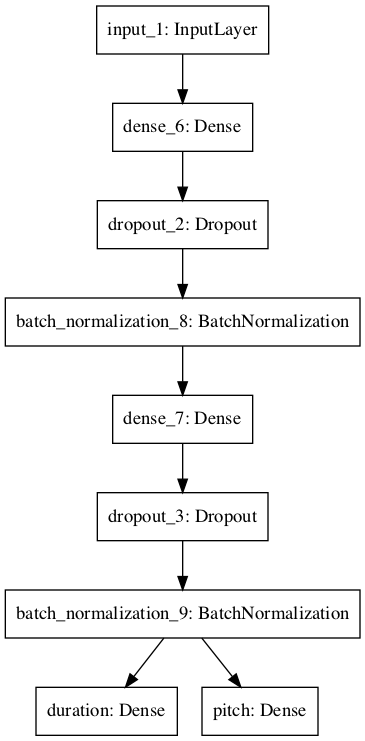
\includegraphics[width=0.3\linewidth]{figure/model_terryjosh} 

}

\caption{museGen Model Structure}\label{fig:unnamed-chunk-2}
\end{figure}
The input of this model is a 128-length vector of standard normal Gaussian noise. The noise will go through 4 dense layers (currently set at 256 nodes each) with ReLU activation, dropout, and batch normalization. Then, the model splits in half, one each for pitch and duration generation. The pitch part of the model then upsamples the output from the last layer into 20*128 nodes, where 20 is for the 20 notes to generate, and 128 is for the one-hot vector of pitches. Similarly, we upsample duration from the same layer into 20*2 nodes, where 20 is for the 20 notes to generate and 2 is for start and end times. Afterwards, we have to reshape these nodes into the correct shapes, (20, 128) for pitches and (20, 2) for duration, and apply to the correct axis the corresponding activation functions: softmax for pitch (for pitch onehot), and ReLU for duration (for outputting positive numbers). The generated pitch and duration vectors are then concacted into one single array of dimensions (20, 130) as the output of the model.

Using this modeling structure, we ensure that pitch and duration of one generated music sample is generated by a single model and one single noise input. The dense layers preceding the split in the model will allow the model to learn latent features and rules of music before feeding that latent representation of the final product into the part of the model that turns latent vectors into pitch and duration.

Conventionally, music generator models are usually time-dependent models such as the LSTM, with some added features like the attention mechanism for model to learn how to place emphasis on repeated patterns. While those models work, they are quite a bit more complex than simple dense neural networks deployed in our approach. We observe that, even with a more simplistic (and thus less artificial) model, the generator is still able to learn basic musical structures.

Once the generator has made its predictions, we have to feed it through another function we wrote to convert the softmax vector for pitch into a one-hot vector, so that the output would look as similar as possible to the real samples.

\hypertarget{discriminator}{%
\subsection*{Discriminator}\label{discriminator}}
\addcontentsline{toc}{subsection}{Discriminator}

Our discriminator model is a simple dense neural network with input dimensions of 20*130 (for the 20 note sample, either generated or real) and outputs a float between 0 and 1 (using sigmoid activation) that represents the probability of whether the sample is fake (0) or real (1).

\textbf{Insert discriminator model image here}

As we can see the model is a straightforward dense neural network (with dropout and batch normalization layers). The model is deliberately kept simplistic here because a big concern during the training was the unequal speeds at which the generator and discriminator learns. More often than not in our case, the discriminator learns much quicker than the generator, and we have concluded that such a simple model actually was the most optimal so that the generator and discriminator can achieve balanced learning for long periods of time.

\hypertarget{adversarial-model}{%
\subsection*{Adversarial Model}\label{adversarial-model}}
\addcontentsline{toc}{subsection}{Adversarial Model}

The adversarial model is simply the sequential collection of the generator and the discriminator as illustrated below:

\textbf{Insert GAN model image here}

However, in the adversarial model, the weights of the discriminator is frozen. The reason for that is the need to feed the error from the discriminator to train the generator. We will expand on this topic in the next section regarding training GAN models.

\hypertarget{training-gan-models}{%
\subsection*{Training GAN models}\label{training-gan-models}}
\addcontentsline{toc}{subsection}{Training GAN models}

Training GAN models is not a straightforward process and requires looping through the following specialized steps:
\begin{enumerate}
\def\labelenumi{\arabic{enumi}.}
\tightlist
\item
  \textbf{Train the discriminator with real samples.} We use a function to sample from the real training data. The size of this sample is usually 1/2 of the batch size parameter of the training script. We then feed this data and the target variable (a vector of 1's) to the discriminator model. The resulting error is the error of misclassificating real samples as fake. We use binary crossentropy as loss metric.
\item
  \textbf{Train the discriminator with fake samples.} We use a function to generate fake samples using the generator model we've set up. The size of this sample is usually 1/2 of the batch size parameter of the training script. We then feed this data and the target variable (a vector of 0's) to the discriminator model. The resulting error is the error of misclassificating fake samples as real. We use binary crossentropy as loss metric.
\item
  \textbf{Train the adversarial model}. We feed the adversarial model with a number of batches of random noise as input, but mark the target variable as a vector of 1's, or telling the model that these are real samples. Since the adversarial is basically the sequential collection of the generator and discriminator, the random noise input will be converted into fake samples of music before getting fed into the discriminator, where the output is a classification of whether the sample is fake or real. Since we are technically mislabeling the data by using 1's as the target variable, the error will negatively correlated with how well the discriminator performs - the the better the discriminator does, the larger the error, thus the more the weights will be adjusted in the generator, and vice versa. The discriminator is not affected because its weights are frozen when training the adversarial model. This serves to balance the rate of learning for the generator and the discriminator and prevents any one of them to become overly good, but this occurs very often in training.
\end{enumerate}
GAN models are notoriously fickle and require special care to train properly \textbf{add footnote}. In our training script, we have set up a mechanism to collect the errors from the discriminator and the generator in order to keep track of training progress and detect any learning issues which happen frequently, and most of our work to date has been to find ways to address these issues. We will address our learning points in the Findings section.

\hypertarget{findings}{%
\chapter*{Findings}\label{findings}}
\addcontentsline{toc}{chapter}{Findings}

We divide our findings into two separate sections: GAN Training and Assessment of Model Output.

\hypertarget{findings-gan_training}{%
\section*{GAN Training}\label{findings-gan_training}}
\addcontentsline{toc}{section}{GAN Training}

GAN models are notoriously hard to train properly. During training of our model, we encountered numerous issues which we have had varying degrees of success in addressing. The main issues are:
\begin{enumerate}
\def\labelenumi{\arabic{enumi}.}
\tightlist
\item
  Loss balancing. In many cases, the errors from the discriminator and generator often collapse to 0 or become extremely large.
\item
  Mode collapse. Model learns to generate one kind of output that is able to fool the discriminator despite random input.
\end{enumerate}
We will be referring to discriminator and generator losses in the following section. To clarify, discriminator loss is loss from training the discriminator specifically and generator loss is the loss from training the adversarial model.

\hypertarget{loss-balancing}{%
\subsection*{Loss Balancing}\label{loss-balancing}}
\addcontentsline{toc}{subsection}{Loss Balancing}

Using the data we collected from the training process, we find that the GAN training can be summarized into three distinctive stages:
\begin{enumerate}
\def\labelenumi{\arabic{enumi}.}
\tightlist
\item
  The initial chaos. The generator and discriminator are trying to balance each other out and the error can vary drastically from epoch to epoch and either the discriminator or generator loss can be much larger than the other. It often settles into a more balanced stage, but this is not a given as we observe some models being unable to get past this initial stage.
\item
  The stable equilibrium. The model enters into a stable stage characterized by similar magnitude of losses between discriminator and generator and across different epochs. Judging from the quality of the output, it is during this period when the model learned the most from training data and generated the most musical samples.
\item
  The final collapse. This stage is characterized by a steady increase in loss magnitude in one of or both the generator and the discriminator, until the losses of either model collapsing to 0. There are even rare cases where both the discriminator and generator losses go down to 0. Learning stops and music generated gets worse and worse.
\end{enumerate}
In the following plot of average epoch losses from one of the training sessions, we can observe these three distinctive stages:
\begin{figure}

{\centering 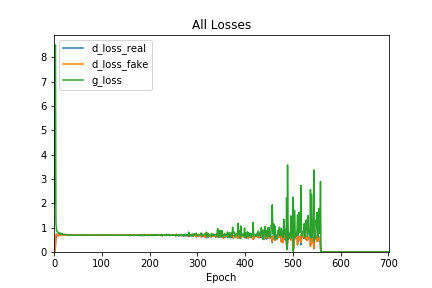
\includegraphics[width=0.3\linewidth]{figure/all_losses_1} 

}

\caption{Training Loss Graph}\label{fig:unnamed-chunk-3}
\end{figure}
During the first 25 epochs or so we observe an initially high but declining losses for both the discriminator and the generator. Thereafter we enter the stable stage that lead to significant and high-quality learning where the loss stablized around 0.7 for both the discriminator and the generator. However, losses become unstable again starting around the 300 to 400 epoch mark and by the 500th epoch the generator loss has increased to around 2 while the discriminator loss is steadily declining. Finally, at around epoch 560, all losses go to zero and the model ceases to learn.

It seems that the model showed the most promise during the stable equilibrium stage. While it is hard to show the quality of the generated samples in a mathematic way, we can clearly demonstrate this by hearing generated samples at different number of epochs. Here is the \href{https://github.com/terrywang15/museG_dev/tree/master/2020-01-31\%2002-20}{link} to our github page to access the generated samples at every 100 epochs during the training session above. At the first epoch, the output from the generator has no sense of rhythm or melody and its output is simply random notes. After 100 epochs, it is clear that there are improvements in rhythm, but the melody is still lacking. At epoch 200 the notes sound much more pleasant as they generally come from the same key. We see more improvement at epoch 300 and 400, which we believe is the best sample generated. However, the improvement trends are reversed starting at epoch 500, and the samples generated become increasingly nonsensical.

This observation shows that the conventional GAN model training procedures that try to balance discriminator and generator learning have much to improve upon, as it fails to prevent the generator to learn how to generate samples that is able to produce zero loss both for the discriminator and at the adversarial stage\footnote{One explanation is that the the fake input to the discriminator when training the discriminator is different from when training the adversarial model: the input to train the discriminator has a preprocess step to take argmax of the softmax vector and make a one-hot vector on the argmax index, meaning that it has the same format as the real samples, but during the adversarial stage this is not the case as the discriminator is fed output from the generator directly without preprocessing. This will be addressed with an update to the model. However, there is also a good chance that there are other reasons for the collapse in losses, as this phenomenon is observed in many other GAN models.}.

It also seems that the loss collapse follows right after the wild oscillations in losses. Since the evidence seems to show that losses stability and generated sample quality are positively correlated, ideally we would want this stage of stable equilibrium to last as long as possible. To achieve that, we can either improve on the model structure, or revise the training procedures. We will discuss some of our ideas for improvement in a later section.

\hypertarget{mode-collapse}{%
\subsection*{Mode Collapse}\label{mode-collapse}}
\addcontentsline{toc}{subsection}{Mode Collapse}

Mode collapse is a common problem for GAN models\footnote{See p113, Generative Deep Learning}. \textbf{maybe figure out correct format for citations} It happens when the generator finds one single pattern that is able to fool the discriminator and then mapping the random noise input to that pattern, so that all outputs from the generator are very similar.

An example of mode collapse is found in one of our training sessions. Judging from the samples, the model seems to learn relatively well during the first few hundred epochs, but starting from epoch 900, the generator will only generate the same sample over and over again. Use this {[}link{]} (\url{https://github.com/terrywang15/museG_dev/tree/master/2020-02-11\%2022-13}) to download and listen to all the samples.

After some investigations, it seems that mode collapse is related to the loss issue described above: mode collapse only happened after all losses collapsed to near zero. Notice in the below graph recording the average epoch losses from the training session that generated the samples mentioned above, the generator started to generate the exact same samples around epoch 900, shortly after the collapse of losses:
\begin{figure}

{\centering 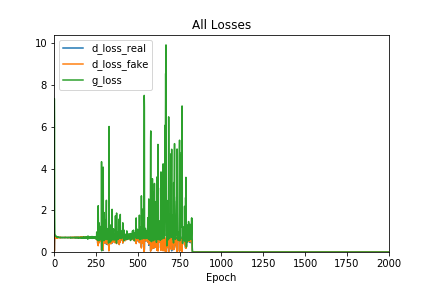
\includegraphics[width=0.3\linewidth]{figure/all_losses_2} 

}

\caption{Training Loss Graph}\label{fig:unnamed-chunk-4}
\end{figure}
It is unknown at this point whether the collapse in losses and mode collapse are related or if we encountered a special case. However, it is clear that we will need to have a mechanism to monitor losses which will indicate to us whether the model is learning effectively.

\hypertarget{ideas-for-improvements-on-model-structure-and-training}{%
\subsection*{Ideas for Improvements on Model Structure and Training}\label{ideas-for-improvements-on-model-structure-and-training}}
\addcontentsline{toc}{subsection}{Ideas for Improvements on Model Structure and Training}

\hypertarget{model-structure-changes-to-separate-pitch-loss-and-duration-loss}{%
\subsubsection*{1. Model Structure Changes to Separate Pitch Loss and Duration Loss}\label{model-structure-changes-to-separate-pitch-loss-and-duration-loss}}
\addcontentsline{toc}{subsubsection}{1. Model Structure Changes to Separate Pitch Loss and Duration Loss}

One hypothesis that we pursued is that having one dedicated generator for pitch and duration would work better than our baseline model. The idea behind this is that, since pitch and duration are very different data types that differ in magnitude when comparing typical losses generated, it would make more sense to separate them so that loss is distributed proportional to how the model performs in terms of pitch and duration. This way, if a model does well in pitch and not duration, for example, the model would devote more losses to duration and less to pitch.

We proceeded to try this idea out, and had one generator each for pitch and duration. However, preliminary results are not very encouraging as the model has so far failed to generate any musical sounding samples.

\hypertarget{change-to-a-different-loss-metric}{%
\subsubsection*{2. Change to a Different Loss Metric}\label{change-to-a-different-loss-metric}}
\addcontentsline{toc}{subsubsection}{2. Change to a Different Loss Metric}

One idea that has worked well in music generation is the Wasserstein loss, which according to its authors is a more meaningful loss metric that correlates better with output quality as well as stablizes the GAN training process\footnote{For details see p115, Generative Deep Learning}. We have yet found time to implement this in our model, so we will leave it as a potential next step.

\hypertarget{automated-monitoring-of-losses-during-training}{%
\subsubsection*{3. Automated Monitoring of Losses During Training}\label{automated-monitoring-of-losses-during-training}}
\addcontentsline{toc}{subsubsection}{3. Automated Monitoring of Losses During Training}

As we have observed, preserving and prolonging the long-term loss stability stage during training should be the goal. We propose to have the following system set up in the training script:
\begin{enumerate}
\def\labelenumi{\arabic{enumi}.}
\tightlist
\item
  Record losses during every batch
\item
  At the end of each epoch, calculate average losses (for generator and discriminator) for that epoch, and record it
\item
  Wait until model ``warms up'' or enters the stable learning stage. We can manually define how this look like or use a metric (such as stationarity)
\item
  Establish a metric for trend stability. This can be the standard deviation of the new epoch's losses compared to the distribution of losses from the stable process
\item
  Stop training when losses shoot up for x number of epochs. We have observed that once the training enters the final collapsing stage it rarely finds its way back, so its better to terminate training rather than keep going in the hopes of finding the stable stage again
\end{enumerate}
\hypertarget{automated-model-structure-changes-during-training}{%
\subsubsection*{4. Automated Model Structure Changes During Training}\label{automated-model-structure-changes-during-training}}
\addcontentsline{toc}{subsubsection}{4. Automated Model Structure Changes During Training}

A more advanced idea that we have been considering is to combine automated loss monitoring with flexible model structures. The idea would go as follows:
\begin{enumerate}
\def\labelenumi{\arabic{enumi}.}
\tightlist
\item
  Make a basic generator/discriminator model with as few layers as possible
\item
  Train model until it enters stable stage
\item
  Monitor losses, stop training when losses start to increase
\item
  Freeze current model weights
\item
  Add new layer to generator and/or discriminator (can have some conditions to trigger this for generator or discriminator)
\item
  Train this new model until loss start to increase. Repeat the process as needed or use a stopping criterion
\end{enumerate}
This way, we hope to maximize learning during the stable stage for each layer while avoiding many of the problems that we have encountered during our training. We believe this is a modeling technique that we should attempt in our next steps.

\hypertarget{findings-assess_model}{%
\section*{Assessment of Model Output}\label{findings-assess_model}}
\addcontentsline{toc}{section}{Assessment of Model Output}

One of the most significant achievements of our generator is that it successfully learned many musical structures despite being fed random snippets of data, demonstrating that GAN model structure is quite flexible in dealing with different forms of data and formats. To illustrate the musicality of generated outputs, we will focus on one generated sample that showed the success of our generator.

The particular sample can be found via this \href{https://github.com/terrywang15/museG_dev/blob/master/2020-01-31\%2002-20/ep_400.mid}{link}. The notes of the sample is shown in the following table:
\begin{longtable}[]{@{}lll@{}}
\caption{\label{tab:inher} Generated Midi Sample 1}\tabularnewline
\toprule
Pitch & Start Time & End Time\tabularnewline
\midrule
\endfirsthead
\toprule
Pitch & Start Time & End Time\tabularnewline
\midrule
\endhead
C5 & 0.000000 & 0.020455\tabularnewline
A3 & 0.000000 & 1.888636\tabularnewline
G4 & 0.000000 & 2.688636\tabularnewline
F\#3 & 0.500000 & 4.229545\tabularnewline
D5 & 2.313636 & 3.797727\tabularnewline
F\#4 & 2.884091 & 2.979545\tabularnewline
G3 & 3.020455 & 6.768182\tabularnewline
E3 & 3.181818 & 3.677273\tabularnewline
D4 & 3.827273 & 4.877273\tabularnewline
D5 & 3.981818 & 4.375000\tabularnewline
E5 & 4.145455 & 4.156818\tabularnewline
C4 & 4.747727 & 5.856818\tabularnewline
E4 & 5.190909 & 6.336364\tabularnewline
A3 & 5.904545 & 6.263636\tabularnewline
C5 & 5.938636 & 7.293182\tabularnewline
E3 & 6.606818 & 7.634091\tabularnewline
B3 & 8.020455 & 8.075000\tabularnewline
D4 & 8.511364 & 8.545455\tabularnewline
\bottomrule
\end{longtable}
When listening to this sample, one can't help but notice how ``musical'' it sounds. This is because it has a structure that adheres to classical western music theory.

The sample begins with an ambiguous chord (A3, G4, C5) which is a transposed version of an A dominant chord with the fifth missing\footnote{There are other interpretations for this chord of course.}, but this chord is abruptly transitioned to the (F\#3, A3, G4) chord, a very dissonant chord that, although jarring, start to pull the song in the direction of a G major/E minor key because of the introduction of the F\# note that is characteristic of the G major/E minor, so overall the beginning sequence establishes the key structure of this sample. The F\#3 note also has a strong tendency to go up a half-step and resolve to G3, which we will learn that it does right after.

The next sequence of notes are very interesting. It starts with the melody line of D5, F\#4, G3, and E3, a remarkably smooth transition that implies D major with the major third as the root (F\#), which transitions to E minor (G3, E3)\footnote{See Circle of Fifths, (\url{https://en.wikipedia.org/wiki/Circle_of_fifths}). The D major chord should transition to G major but can also transition to E minor.}. There are several remarkable things happening here: first, the generator chooses a melody line that spans a wide range of octaves, giving it a sound that is very characteristic of piano music; second, the melody smartly includes the note G3, which serves the dual purpose of resolving the jarring F\#3 note from the beginning sequence and anticipating the next chord (E minor).

After this sequence, the sample has firmly established an E minor feel. Next, it features an additional transition to C major then A minor through a very interesting setup (D4, D5, E5, C4, E4, A3). The octave-skipping D notes at the beginning is again found in many piano music and serves to reinforce the the D note, a note that clashes somewhat with the E minor chord the sample is in at that point and has a tendency to resolve to E or go down to C. After introducing this tension, the sample deftly does both of these things: the leading D5 goes up to E5 as a glide, the D4 goes down to C4, exactly what we would expect. But notice how the two resolutions went in different directions: D4 went down a step, while D5 went up a step. This kind of arrangement is very common in Baroque era music, which generally shuns multiple voices moving in parallel\footnote{See Counterpoint, (\url{https://en.wikipedia.org/wiki/Counterpoint})}. Finally, an E4 is played after C4 to anchor the chord with a major third and removing ambiguities to what the implied chord is. This is followed by an A3 note which is again a smooth transition because it transitions to a new chord (A minor) by only adding one note (A3) while keeping the other notes (C4, E4) the same.

The ending sequence also features an interesting movement that could be interpreted as an attempt to make a key change in the context. The note sequence (C5, E3, B3, D4) can be understood as an attempt to move from the A minor or C major to a B major. Either way, it would entail a parallel shift of voices up or down a whole step, something that Baroque does not like. The generator's solution to this problem is to spread out the the two voices by almost 2 octaves (C5, E3) then bringing them together closer, with the C5 moving down to D4 and E3 moving up to B3. Also, the kind of resolving chords to something a half step lower (C chord to B chord) is commonly heard in Jazz and certainly makes sense in music theory. The reason that this sounds like a transition to a different key is because B is never heard throughout the sample up to that point, in addition to the sudden break in rhythmic pattern.

Speaking of rhythms, this generated sample also seems to have learned to produce coherent rhythmic structure. For example, in this sample melody line (D5, F\#4, G3, E3) has a rhythmic pattern consisting of a long note followed by several short notes. The next melody line (D4, D5, E5, C4) references the structure of the preceding notes by reversing it: it now has several short notes followed by a long note. This kind of rhythmic construction is what gives a melody line a ``human'' feel, because it creates a pattern that repeats itself and at the same time is different in each repetition. Moreover, the rhythm and melody seem to work extremely well together, showing the success of our model structure which generates pitches and duration from the same latent space.

We now can see how the generator under the GAN structure achieved outputs of the following:
\begin{enumerate}
\def\labelenumi{\arabic{enumi}.}
\tightlist
\item
  It learned basic music theory such as keys and chords;
\item
  It learned what rhythm sounds natural
\item
  It learned to consider past and future notes as a whole and try to create repeated patterns;
\item
  It learned highly abstract ideas such as chord progression and avoidance of clashing voices.
\end{enumerate}
Even more remarkable is how this is achieved without relying on explicitly encoding any artificial structures, such as LSTM or the Attention mechanism, in the generator in order to ``force'' the model to learn self-referencing behavior and pattern recognition. It shows the remarkable flexibility of the deep neural network architecture. At the same time, more attention must be paid on the training steps in order for this model to learn as much useful information as possible.

\hypertarget{conclusion}{%
\chapter*{Conclusion}\label{conclusion}}
\addcontentsline{toc}{chapter}{Conclusion}

This section includes a concise summary of the findings. Your summary might be organized by the research objectives or hypotheses. Make sure you address the extent to which research objectives are achieved, and if they are not achieved, explain why. Make sure to interpret your findings in a way that acknowledges the limitations of the research. That is, do not extrapolate the insights derived from your research to situations you have not examined.

\emph{While increasing dosage leads to larger incisor length, the choice of delivery mechanism between Orange Juice and Vitamin C does not seem to make a difference. However, at very low levels, Orange Juice appears more effective, displaying higher average growth.}

\hypertarget{recommendations}{%
\chapter*{Recommendations}\label{recommendations}}
\addcontentsline{toc}{chapter}{Recommendations}

Includes guidelines as to ways in which your results should or could be used in practice. You may discuss other uses of your results, if there are any. The ways to extend your analysis and the benefits of doing so might be included in this section as well.

\appendix

\hypertarget{the-first-appendix}{%
\chapter{The First Appendix}\label{the-first-appendix}}

This first appendix includes all of the R chunks of code that were hidden throughout the document (using the \texttt{include\ =\ FALSE} chunk tag) to help with readibility and/or setup.

\textbf{In section} \ref{pressure-plot}:

\textbf{In section \ref{ref-labels}:}

\hypertarget{a-second-appendix-for-example}{%
\chapter{A Second Appendix, for example}\label{a-second-appendix-for-example}}

\backmatter

\hypertarget{references}{%
\chapter*{References}\label{references}}
\addcontentsline{toc}{chapter}{References}

\markboth{References}{References}

\noindent

\setlength{\parindent}{-0.20in}
\setlength{\leftskip}{0.20in}
\setlength{\parskip}{8pt}

There are a variety of tools available for creating a bibliography database (stored with the .bib extension). In addition to BibTeX suggested below, you may want to consider using the free and easy-to-use tool called \href{https://www.zotero.org/}{Zotero}.

\emph{R Markdown} uses \emph{pandoc} (\url{http://pandoc.org/}) to build its bibliographies. To cite references in your thesis (after creating your bibliography database), place the reference name inside square brackets and precede it by the ``at'' symbol. For example, here's a reference to a book about worrying: (Molina \& Borkovec, 1994). This \texttt{Molina1994} entry appears in a file called \texttt{thesis.bib} in the \texttt{bib} folder. This bibliography database file was created by a program called BibTeX. You can call this file something else if you like (look at the YAML header in the main .Rmd file) and, by default, is to placed in the \texttt{bib} folder.

\textbf{Additional Tips}
\begin{itemize}
\tightlist
\item
  The sooner you start compiling your bibliography for something as large as a capstone, the better. Typing in source after source is mind-numbing enough; do you really want to do it for hours on end at the last minute?
\item
  The cite key (a citation's label) needs to be unique from the other entries.
\item
  When you have more than one author or editor, you need to separate each author's name by the word ``and'' e.g. \texttt{Author\ =\ \{Noble,\ Sam\ and\ Youngberg,\ Jessica\},}
\end{itemize}
\textbf{Example output generated from bib file}

\hypertarget{refs}{}
\leavevmode\hypertarget{ref-angel2000}{}%
Angel, E. (2000). \emph{Interactive computer graphics : A top-down approach with opengl}. Boston, MA: Addison Wesley Longman.

\leavevmode\hypertarget{ref-angel2001}{}%
Angel, E. (2001a). \emph{Batch-file computer graphics : A bottom-up approach with quicktime}. Boston, MA: Wesley Addison Longman.

\leavevmode\hypertarget{ref-angel2002a}{}%
Angel, E. (2001b). \emph{Test second book by angel}. Boston, MA: Wesley Addison Longman.

\leavevmode\hypertarget{ref-Molina1994}{}%
Molina, S. T., \& Borkovec, T. D. (1994). The Penn State worry questionnaire: Psychometric properties and associated characteristics. In G. C. L. Davey \& F. Tallis (Eds.), \emph{Worrying: Perspectives on theory, assessment and treatment} (pp. 265--283). New York: Wiley.


% Index?

\end{document}
